\section{Evaluation}

For the three base types of controllers, P, PI and PID, different characteristic parameters are used. The procedure was carried on with various setpoints which portrayed the operating points. The graphs part show the different experiments:
TODO: Text Yohannes

\subsection{P-Controller}
In the following three sections, the Ziegler-Nichols method was used. For that, \textbf{$K_{P,rule}$} $= 0.7$ was used. For the actual controller, $K_P$ was a modification of $K_{P,rule}$.


In the experiment of the P-controller shows that the deviation of the error decreases with the increasing of $K_{p}$.

First, a controller with
\begin{center}
{$K_{p}= K_{P,rule}\cdot{0.2}$}
\end{center}

was used. One can clearly see in Figure \ref{fig:p_controller2} that the deviation from the setpoint is huge.

\begin{figure}[H]
\begin{center}
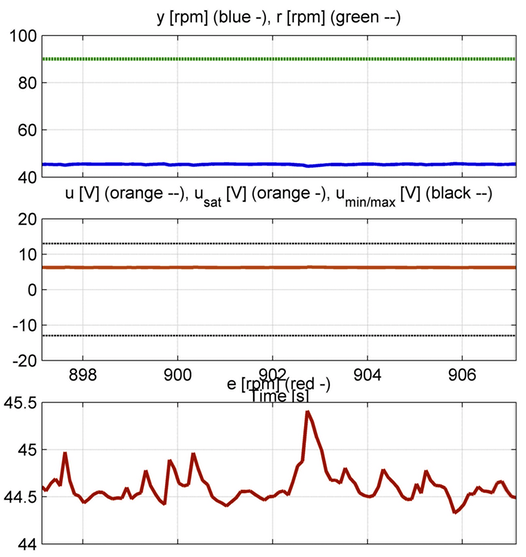
\includegraphics[width=0.5\linewidth]{images/general/P/p_controller02}
\end{center}
\caption{P-Controller of $ K_{P,rule}*\cdot{0.2}$}
\label{fig:p_controller2}
\end{figure}

To narrow the gap from the actual output to the set-point, a new value for $K_P$ was used:

\begin{center}
{$K_{p}= K_{P,rule}$}
\end{center}

The error is now much smaller as obtained in Figure \ref{fig:p_controller1}, but still a good 15\% off to the actual setting point.

\begin{figure}[H]
\begin{center}
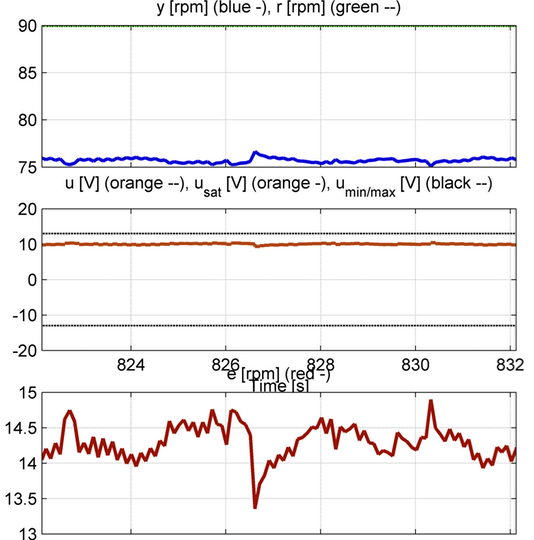
\includegraphics[width=0.5\linewidth]{images/general/P/p_controller1}
\end{center}
\caption{P-Controller of $ K_{P,rule}$}
\label{fig:p_controller1}
\end{figure}

Since the error decreased with increasing $K_P$, an even bigger value was tested:

\begin{center}
{$K_{p}= K_{P,rule}\cdot4$}
\end{center}

Considering Figure \ref{fig:p_controller4} the error did indeed decrease even more. Sadly now the actual value started to oscillate. To counteract this, in a next step, a PI-Controller will be tested.

\begin{figure}[H]
\begin{center}
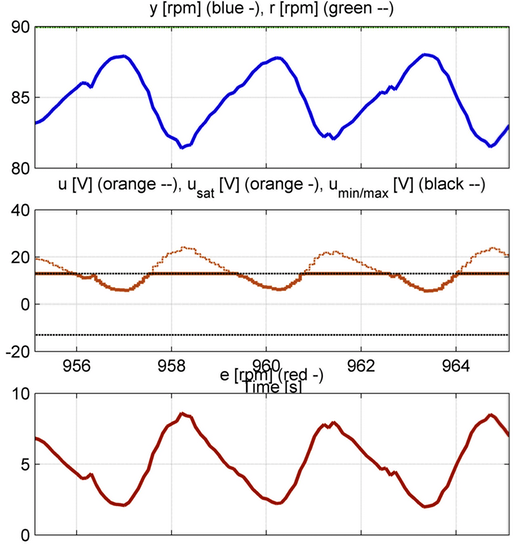
\includegraphics[width=0.5\linewidth]{images/general/P/p_controller4}
\end{center}
\caption{P-Controller of $ T_{T,rule}\cdot{4}$}
\label{fig:p_controller4}
\end{figure}
\clearpage

\subsection{PI-Controller}

In this experiment, the increase of $T_{i}$ should reduce the overshoot but in the same time increase the time used to reach the set-point whereas the decrease of $ T_{i}$ should reincrease oscillation with fast rise time that forces the controller to reach the setpoint in a much shorter time.
Onse again the Ziegler-Nichols method was used.

At first an experiment with
\begin{center}
{$K_{p}= K_{P,rule}$ and $ T_{i,rule}\cdot0.2$}
\end{center}

was carried out. As seen in Figure \ref{fig:PI_Controller02} the RMS deviation from the setting point nearly vanished. Sadly the system still oscillates a lot.

\begin{figure}[H]
\begin{center}
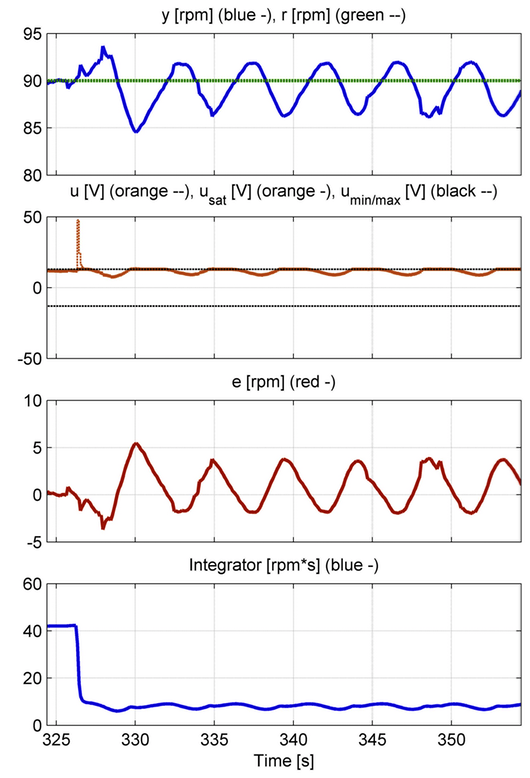
\includegraphics[width=0.5\linewidth]{images/general/PI/PI_Controller02}
\end{center}
\caption{P-Controller of $ T_{i,rule}\cdot{0.2}$}
\label{fig:PI_Controller02}
\end{figure}


From Figure \ref{fig:PI_RiseTime02} the rise time for the above controller configuration can be extracted. It is quite some time which can surely be decreased.

\begin{figure}[H]
\begin{center}
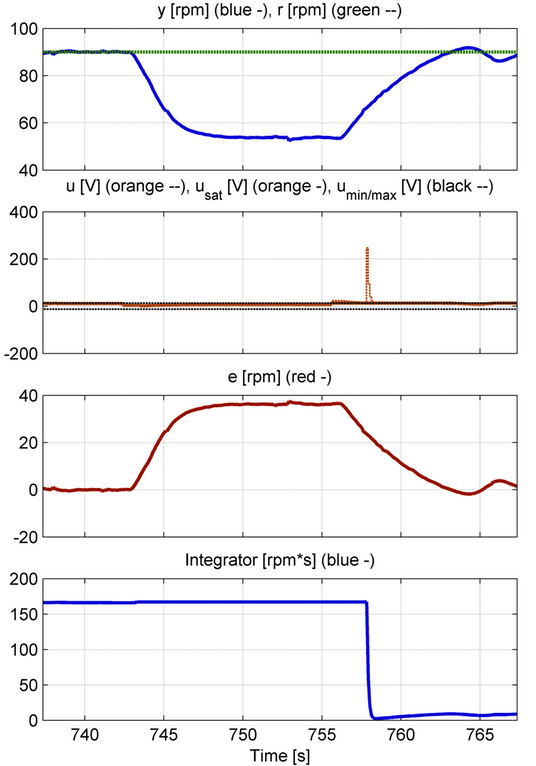
\includegraphics[width=0.5\linewidth]{images/general/PI/PI_RiseTime02}
\end{center}
\caption{P-Controller of $ T_{I,rule}\cdot{0.2}$}
\label{fig:PI_RiseTime02}
\end{figure}

Now the paramters were set to

\begin{center}
{$K_{p}= K_{p,rule}$ and $T_{i}=T_{i,rule}$}
\end{center}

In Figure \ref{fig:PI_Controller1} it can be observed that the error has now close to vanished. Sometimes the output still spikes but that can also be measurement errors.

\begin{figure}[H]
\begin{center}
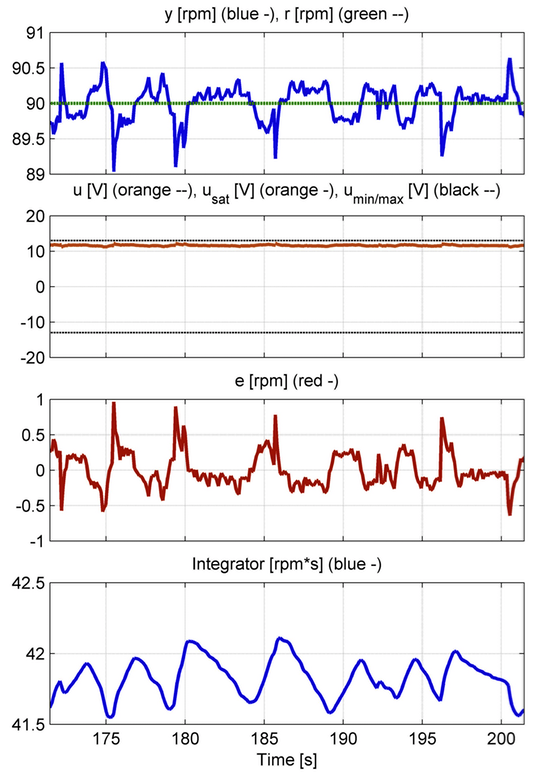
\includegraphics[width=0.5\linewidth]{images/general/PI/PI_Controller1}
\end{center}
\caption{P-Controller of $ T_{i,rule}$}
\label{fig:PI_Controller1}
\end{figure}

The rise time is still about the same as before, as seen in Figure \ref{fig:PI_RiseTime1}.

\begin{figure}[H]
\begin{center}
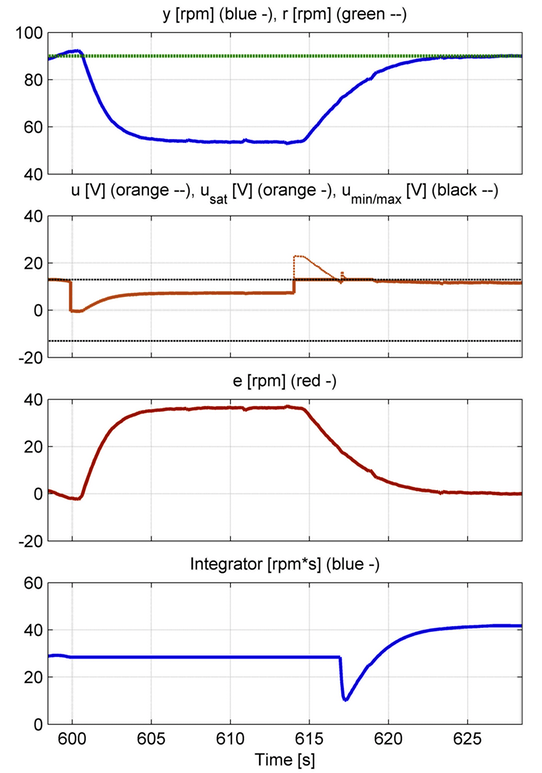
\includegraphics[width=0.5\linewidth]{images/general/PI/PI_RiseTime1}
\end{center}
\caption{P-Controller of $ T_{i,rule}$}
\label{fig:PI_RiseTime1}
\end{figure}

Last but not least the values

\begin{center}
{$K_{p}= K_{P,rule}$ and $T_{i}=T_{i,rule}\cdot4$}
\end{center}

were tested. The error did not worsen but the rise time quadrupled!
(Consult Figures \ref{fig:PI_Controller4} and \ref{fig:PI_RiseTime4})
This is not wanted and a lower $T_i$ should be selected for sure.

\begin{figure}[H]
\begin{center}
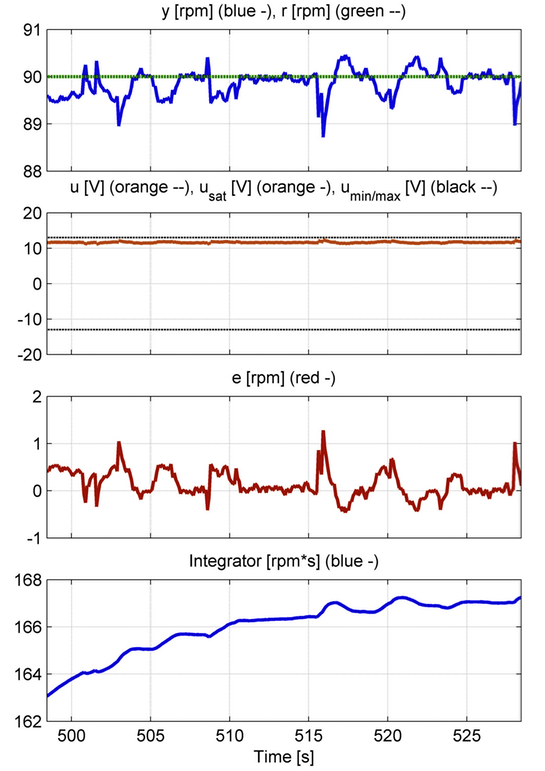
\includegraphics[width=0.5\linewidth]{images/general/PI/PI_Controller4}
\end{center}
\caption{P-Controller of $ K_{P,rule}\cdot4$}
\label{fig:PI_Controller4}
\end{figure}

\begin{figure}[H]
\begin{center}
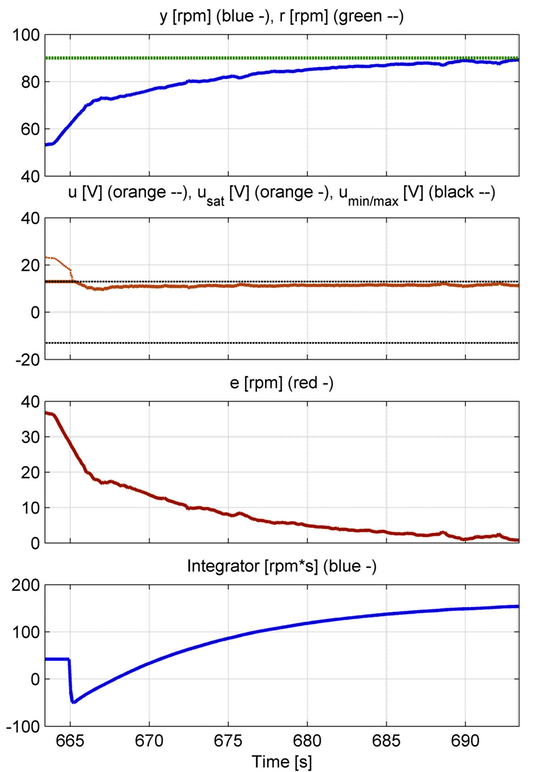
\includegraphics[width=0.5\linewidth]{images/general/PI/PI_RiseTime4}
\end{center}
\caption{P-Controller of $ K_{P,rule}\cdot4$}
\label{fig:PI_RiseTime4}
\end{figure}

\clearpage
\subsection{PID-Controller}

To improve the behavior of the controller even more, a full PID controller was tested now.
Both, the Ziegler-Nichols and Chien-Hrones-Reswick methods of tuning PID controllers have been used for the following part of the experiment. 

To carry out the experiment using the Ziegler-Nichols method, the values in Table \ref{tab:zn_params} were used.
The resulting behavior can be observed in Figure \ref{fig:Ziegler_nichols}

\begin{table}[H]
\begin{center}
\begin{tabular}{ |c|c| } 
 \hline
 Parameter & Value\\
 \hline
 $T_{d}$ & 0.32\\  
 \hline
 $T_{i}$ & 1.33\\
 \hline
 $K_{p}$ & 0.84\\
 \hline
\end{tabular}
\end{center}
\caption{Ziegler-Nichols Parameter}
\label{tab:zn_params}
\end{table}

\begin{figure}[H]
\begin{center}
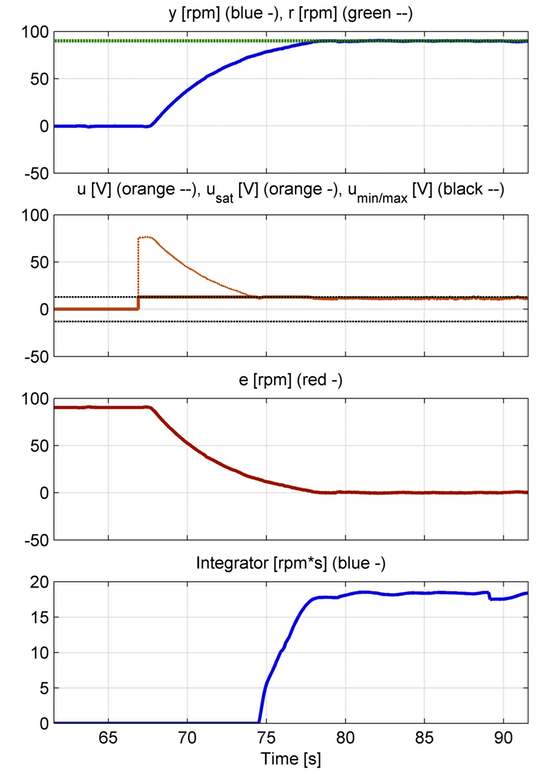
\includegraphics[width=0.5\linewidth]{images/general/PID/Ziegler_nichols}
\end{center}
\caption{Ziegler-nichols tuning rule for $T_{i}, T_{d},K_{P}$}
\label{fig:Ziegler_nichols}
\end{figure}

For the Chien, Hrones, Reswick experiment, the values in Table \ref{tab:chr_params} were used.

\begin{table}[H]
\begin{center}
\begin{tabular}{ |c|c| } 
 \hline
 Parameter & Value\\
 \hline
 $T_{d}$ & 0.5\\  
 \hline
 $T_{i}$ & 2\\
 \hline
 $K_{p}$ & 0.154\\
 \hline
\end{tabular}
\end{center}
\caption{Chien, Hrones, Reswick Parameter}
\label{tab:chr_params}
\end{table}

The systems behavior using these parameters can be studied in Figure \ref{fig:Chien_Hrones_Reswick}

\begin{figure}[H]
\begin{center}
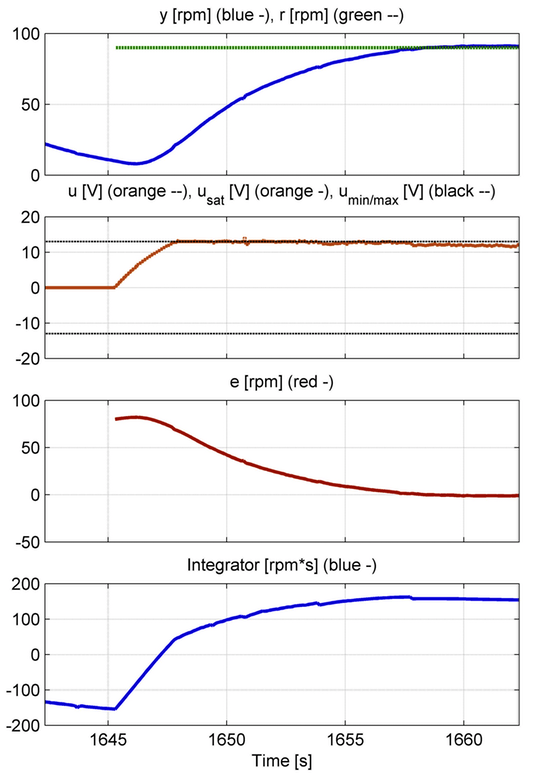
\includegraphics[width=0.5\linewidth]{images/general/PID/Chien_Hrones_Reswick}
\end{center}
\caption{Chien-Hrones-Reswick tuning rule for $T_{i}, T_{d},K_{P}$}
\label{fig:Chien_Hrones_Reswick}
\end{figure}

Both methods of creating a controller yielded similar results. It was then decided to go with the Chien, Hrones, Reswick approach and tinker with it and try and optimize the resulting controller.
Sadly the rise time could not really be reduced. For that to happen $T_i$ possibly should have been reduced a lot more whilst the $K_P$ and $T_d$ should have increased a lot.
The disturbance rejection capability is okay, but the system is still very prone to disturbances. This behavior can be seen in Figure \ref{fig:error_rejection}

\begin{figure}[H]
\begin{center}
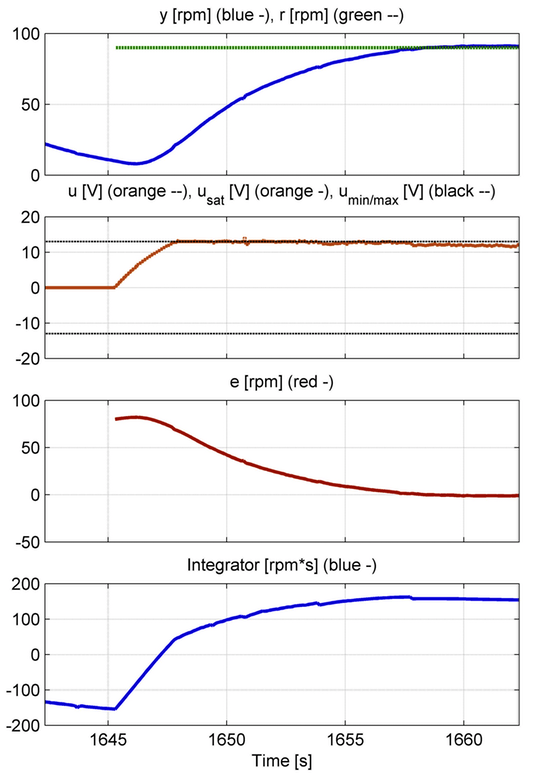
\includegraphics[width=0.5\linewidth]{images/general/PID/Chien_Hrones_Reswick}
\end{center}
\caption{Error rejection of the tuned controller}
\label{fig:error_rejection}
\end{figure}